% =============================================================================
% ICAITech 2026 — Benchmarking Keyword Spotting on Raspberry Pi 5
% Style: Mid-Century Modern Beamer Theme (adapted from deck/demo.tex)
% Compile with: tectonic slides.tex
% =============================================================================
\documentclass[aspectratio=169]{beamer}

\usepackage{beamerthememidcenturymodern}
\usepackage{booktabs}
\usepackage{array}
\usepackage{tikz}

% --- Theme selection ---
% Built-in options: DeepBlue (navy & crisp cyan) or Kraft (terracotta & warm tones)
\mcmTheme{DeepBlue}
% \mcmTheme{Kraft}

% Compact block spacing for dense data slides
\setlength{\mcmBlockSep}{0.45em}
\setlength{\mcmBlockPad}{0.35em}

% --- Metadata ---
\title[Benchmarking KWS on Raspberry Pi 5]{%
  Benchmarking Keyword Spotting Architectures across TensorFlow Lite and ONNX Runtime on a Raspberry Pi 5}

\subtitle{2026 8th International Conference on Artificial Intelligence and Information Technology (ICAITech)}

\author[Fatih \& Amirul]{%
  \textbf{Fatih Jawwad Al Mumtaz}$^{1}$ \and \textbf{Amirul Al Aziz}$^{2}$}

\institute[]{
  Faculty of Science and Technology, Universitas Darussalam Gontor, Indonesia\\[0.3ex]
  \texttt{\scriptsize fatihalmumtaz76@student.cs.unida.gontor.ac.id \quad amirulalaziz57@student.tip.unida.gontor.ac.id}\\[0.4ex]
  \textbf{\scriptsize Zenodo DOI: 10.5281/zenodo.23765521 \quad | \quad License: GNU AGPLv3}
}

\date{ICAITech 2026}

\begin{document}

% =============================================================================
% SLIDE 1: Title Page
% =============================================================================
\begin{frame}[plain]
  \logo{
\includegraphics[height=1.05cm]{logo.png}}
  \titlepage
\end{frame}

% =============================================================================
% SLIDE 2: Context & Motivation
% =============================================================================
\begin{frame}{Context \& Motivation}
\framesubtitle{Always-On Voice at the Extreme Edge}
\begin{columns}[T]
  \begin{column}{0.48\textwidth}
    \begin{block}{The Edge KWS Workload}
      \begin{itemize}\small
        \item \textbf{Always-On Audio}: Continuously scans audio for wake-words.
        \item \textbf{Canonical Benchmark}: Standard task in MLPerf Tiny suite.
        \item \textbf{Strict Constraints}: Sub-millisecond latency ($<1$\,ms) and mW power.
      \end{itemize}
    \end{block}
  \end{column}

  \begin{column}{0.48\textwidth}
    \begin{exampleblock}{Why On-Device? (SDG 3 Alignment)}
      \begin{itemize}\small
        \item \textbf{Zero Cloud Dependency}: Works in offline rural clinics.
        \item \textbf{Strict Audio Privacy}: Biometric voice data never leaves device.
        \item \textbf{Target 3.8}: Hands-free assistive tech for patient diagnostics.
      \end{itemize}
    \end{exampleblock}
  \end{column}
\end{columns}

\begin{alertblock}{The Deployment Question}
  \small TinyML literature routinely assumes \textbf{TensorFlow Lite (TFLite)} is the fastest runtime on Arm. But on 64-bit Arm SBCs (Pi 5 Cortex-A76), \textbf{is TFLite universally faster than ONNX Runtime across diverse architectures?}
\end{alertblock}
\end{frame}

% =============================================================================
% SLIDE 3: Benchmark Model Zoo & Fair Reconstruction
% =============================================================================
\begin{frame}{Benchmark Model Zoo}
\framesubtitle{Front-End Standardization \& Fair Reconstruction}
All models consume an identical \textbf{$49 \times 10 \times 1$ MFCC frame} and output a \textbf{12-way softmax}.

\vspace{0.1em}
\begin{table}[h]
\centering
\scriptsize
\setlength{\tabcolsep}{4pt}
\begin{tabular}{llp{9.0cm}}
\toprule
\textbf{Model} & \textbf{Params} & \textbf{Structural Summary} \\
\midrule
\textbf{DS-CNN (MLPerf Ref.)} & 22,604 & Conv $10\times4$ (stride 2) + 4 $\times$ (DW $3\times3$ + PW $1\times1$) + GAP + Dense \\
\textbf{DNN (Baseline)}        & 88,396 & 4-layer MLP: 490--128--128--64--12 (lower-bound anchor) \\
\textbf{LSTM (Compact)}        & 19,980 & Unrolled LSTM(64) over 49 time-steps + Dense head \\
\textbf{CRNN (Hybrid)}         & 56,844 & Conv $3\times3$ ($\times2$) + MaxPool ($\times2$) + Unrolled GRU(64) + Dense \\
\bottomrule
\end{tabular}
\end{table}

\begin{columns}[T]
  \begin{column}{0.48\textwidth}
    \begin{block}{Decompiling Mixed-Precision MLPerf}
      \small The official MLPerf reference is actually \textbf{mixed-precision} (int8 conv, fp32 remainder). We decompiled and rebuilt a true-fp32 model for fair cross-runtime export.
    \end{block}
  \end{column}
  \begin{column}{0.48\textwidth}
    \begin{exampleblock}{Full INT8 Post-Training Quantization}
      \small Re-quantized with 1,000 representative clips (seed 42) into \textbf{true full-int8} flatbuffers (float I/O, int8 internal GEMM/conv operators).
    \end{exampleblock}
  \end{column}
\end{columns}
\end{frame}

% =============================================================================
% SLIDE 4: Controlled Benchmark Protocol on Raspberry Pi 5
% =============================================================================
\begin{frame}{Experimental Rigor}
\framesubtitle{Controlled Benchmark Protocol on Raspberry Pi 5}
\begin{columns}[T]
  \begin{column}{0.48\textwidth}
    \begin{block}{Hardware \& OS Environment}
      \begin{itemize}\small
        \item \textbf{SoC}: Broadcom BCM2712 (Raspberry Pi 5)
        \item \textbf{CPU}: Quad-core Arm Cortex-A76 @ 2.4 GHz
        \item \textbf{RAM}: 8 GB LPDDR4X (synchronous)
        \item \textbf{OS}: Debian 64-bit GNU/Linux (Kernel 6.18)
        \item \textbf{Governor}: Pinned to \texttt{performance}
        \item \textbf{Runtimes}: LiteRT 2.1.6 vs ONNX Runtime 1.28
      \end{itemize}
    \end{block}
  \end{column}

  \begin{column}{0.48\textwidth}
    \begin{block}{Statistical Protocol}
      \begin{itemize}\small
        \item \textbf{Warmup}: 1,000 unmeasured consecutive passes
        \item \textbf{Sampling}: 1,000 sequential passes (never interleaved)
        \item \textbf{Outliers}: Filtered via 1.5 $\times$ IQR rule
        \item \textbf{Bootstrapping}: 10,000 resamples for 95\% CIs
        \item \textbf{Dual Test Sets (Speech Commands v2)}:
          \begin{itemize}\footnotesize
            \item \textbf{10-Command Subset}: 4,074 official clips
            \item \textbf{Full 12-Class Task}: 12,005 clips (+unknown/silence)
          \end{itemize}
      \end{itemize}
    \end{block}
  \end{column}
\end{columns}
\end{frame}

% =============================================================================
% SLIDE 5: Accuracy Results
% =============================================================================
\begin{frame}{Accuracy Evaluation}
\framesubtitle{10-Command Subset vs Full 12-Class Task}
\begin{table}[h]
\centering
\scriptsize
\setlength{\tabcolsep}{5pt}
\begin{tabular}{lcccccc}
\toprule
& \multicolumn{3}{c}{\textbf{10-Command Subset (4,074 clips)}} & \multicolumn{3}{c}{\textbf{Full 12-Class Task (12,005 clips)}} \\
\cmidrule(lr){2-4} \cmidrule(lr){5-7}
\textbf{Model} & \textbf{fp32 (\%)} & \textbf{int8 (\%)} & \textbf{$\Delta$ (pts)} & \textbf{fp32 (\%)} & \textbf{int8 (\%)} & \textbf{$\Delta$ (pts)} \\
\midrule
\textbf{DS-CNN (ref.)} & 90.55 & 90.57 & \textbf{+0.02} & 95.49 & 95.21 & \textbf{$-$0.28} \\
\textbf{DNN (anchor)}   & 79.63 & 79.65 & \textbf{+0.02} & 72.65 & 71.90 & \textbf{$-$0.75} \\
\textbf{LSTM}          & 90.48 & 87.43 & \textbf{$-$3.05} & 88.84 & 84.72 & \textbf{$-$4.12} \\
\textbf{CRNN}          & \textbf{92.56} & \textbf{92.17} & \textbf{$-$0.39} & \textbf{92.08} & \textbf{91.60} & \textbf{$-$0.48} \\
\bottomrule
\end{tabular}
\end{table}

\begin{columns}[T]
  \begin{column}{0.31\textwidth}
    \begin{exampleblock}{Numerical Parity}
      \scriptsize TFLite fp32 and ONNX fp32 match top-1 classifications across all 12,005 clips (diff $<3\times 10^{-6}$).
    \end{exampleblock}
  \end{column}
  \begin{column}{0.33\textwidth}
    \begin{alertblock}{Recurrent PTQ Cost}
      \scriptsize LSTM suffers large drop (\textbf{$-$4.12 pts} on full task), proving recurrence is hard to quantize without QAT.
    \end{alertblock}
  \end{column}
  \begin{column}{0.31\textwidth}
    \begin{block}{CNN Resilience}
      \scriptsize DS-CNN and CRNN lose $<0.5$\,pts on the full task, demonstrating high robustness to full-int8 PTQ.
    \end{block}
  \end{column}
\end{columns}
\end{frame}

% =============================================================================
% SLIDE 6: Latency Results & Reversal
% =============================================================================
\begin{frame}{Latency Benchmark}
\framesubtitle{The Architecture Reversal Phenomenon}
\begin{columns}[T]
  \begin{column}{0.51\textwidth}
    \begin{table}[h]
    \centering
    \scriptsize
    \setlength{\tabcolsep}{3pt}
    \begin{tabular}{lcccc}
    \toprule
    \textbf{Model} & \textbf{TFLite} & \textbf{INT8} & \textbf{ONNX} & \textbf{Speedup} \\
    \midrule
    \textbf{DS-CNN} & 0.2107 & \textbf{0.1268} & \textbf{0.1702} & \textbf{0.81$\times$} (ONNX) \\
    \textbf{DNN}    & \textbf{0.0158} & \textbf{0.0067} & 0.0286 & \textbf{1.81$\times$} (TFLite) \\
    \textbf{LSTM}   & \textbf{0.3722} & \textbf{0.1569} & 0.7782 & \textbf{2.09$\times$} (TFLite) \\
    \textbf{CRNN}   & \textbf{0.2586} & \textbf{0.1016} & 0.3609 & \textbf{1.40$\times$} (TFLite) \\
    \bottomrule
    \end{tabular}
    \end{table}

    \begin{block}{Key Architectural Insight}
      \begin{itemize}\scriptsize
        \item \textbf{Why ONNX wins on DS-CNN}: Operator-dispatch bound. ONNX fuses depthwise and pointwise convolution kernels.
        \item \textbf{Why TFLite wins on others}: GEMM and sequential bound. TFLite's lightweight session machinery wins by \textbf{1.40--2.09$\times$}.
      \end{itemize}
    \end{block}
  \end{column}

  \begin{column}{0.46\textwidth}
    \centering
    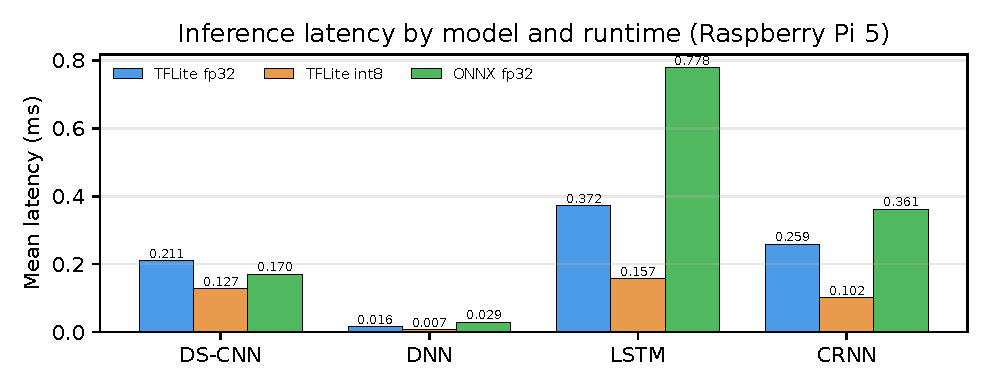
\includegraphics[width=\linewidth]{figures/latency_multi.pdf}
    \vspace{-0.4em}
    \begin{exampleblock}{Full INT8 Acceleration}
      \scriptsize Full-int8 DS-CNN executes in \textbf{0.1268\,ms} (25\% faster than ONNX fp32 and mixed-precision artifact).
    \end{exampleblock}
  \end{column}
\end{columns}
\end{frame}

% =============================================================================
% SLIDE 7: Thread Sensitivity Sweep
% =============================================================================
\begin{frame}{Thread-Sensitivity Sweep}
\framesubtitle{Deconfounding Multi-Thread Defaults (T = 1, 2, 4 Cores)}
\begin{columns}[T]
  \begin{column}{0.48\textwidth}
    \begin{table}[h]
    \centering
    \scriptsize
    \setlength{\tabcolsep}{3pt}
    \begin{tabular}{lccc}
    \toprule
    \textbf{Model \& Runtime} & \textbf{T=1} & \textbf{T=2} & \textbf{T=4} \\
    \midrule
    \textbf{DS-CNN TFLite} & 0.2119 & 0.1229 & \textbf{0.0782} \\
    \textbf{DS-CNN ONNX}   & 0.4379 & 0.2594 & 0.1689 \\
    \textit{Ratio (ONNX / TFLite)} & \textbf{2.07$\times$} & \textbf{2.11$\times$} & \textbf{2.16$\times$} \\
    \midrule
    \textbf{CRNN TFLite}   & 0.2598 & \textbf{0.1873} & 0.2195 \\
    \textbf{CRNN ONNX}     & 0.5075 & 0.4186 & 0.3610 \\
    \textit{Ratio (ONNX / TFLite)} & \textbf{1.95$\times$} & \textbf{2.24$\times$} & \textbf{1.64$\times$} \\
    \bottomrule
    \end{tabular}
    \end{table}

    \begin{alertblock}{The Threading Confound}
      \small Default ONNX silently spawned a \textbf{4-thread pool}, while TFLite ran on \textbf{1 thread}!
    \end{alertblock}
  \end{column}

  \begin{column}{0.48\textwidth}
    \begin{block}{Controlled Iso-Thread Results}
      \begin{itemize}\small
        \item \textbf{TFLite Wins at Every Thread Count}: Pinned to $T=1$, TFLite is \textbf{2.07$\times$ faster} than ONNX on DS-CNN (0.2119 vs 0.4379\,ms).
        \item \textbf{Diminishing Returns on Small Models}: CRNN at 4 threads is slower than at 2 threads due to thread synchronization overhead.
        \item \textbf{Ranking Preserved}: The relative architecture ranking is completely preserved across core sweeps.
      \end{itemize}
    \end{block}
  \end{column}
\end{columns}
\end{frame}

% =============================================================================
% SLIDE 8: On-Board PMIC Energy Measurement
% =============================================================================
\begin{frame}{On-Board SoC Energy Profiling}
\framesubtitle{PMIC ADC Telemetry \& The Race-to-Sleep Paradox}
\begin{columns}[T]
  \begin{column}{0.48\textwidth}
    \begin{table}[h]
    \centering
    \scriptsize
    \setlength{\tabcolsep}{3pt}
    \begin{tabular}{lcccc}
    \toprule
    \textbf{Model} & \textbf{Runtime} & \textbf{$P_\Delta$ (W)} & \textbf{$t_\text{lat}$ (ms)} & \textbf{Energy $E$} \\
    \midrule
    \textbf{DS-CNN} & \textbf{TFLite fp32} & 1.59 & 0.217 & \textbf{0.34 mJ} \\
    \textbf{DS-CNN} & ONNX fp32   & 1.18 & 0.448 & 0.53 mJ \\
    \midrule
    \textbf{CRNN}   & \textbf{TFLite fp32} & 1.85 & 0.274 & \textbf{0.51 mJ} \\
    \textbf{CRNN}   & ONNX fp32   & 1.58 & 0.494 & 0.78 mJ \\
    \midrule
    \textbf{LSTM}   & \textbf{TFLite fp32} & 1.81 & 0.406 & \textbf{0.74 mJ} \\
    \textbf{LSTM}   & ONNX fp32   & 1.31 & 0.725 & 0.95 mJ \\
    \bottomrule
    \end{tabular}
    \end{table}

    \begin{block}{Direct On-Chip ADC Telemetry}
      \small Captured via \texttt{vcgencmd pmic\_read\_adc} across 12 voltage rails. Measures pure SoC energy, excluding peripherals.
    \end{block}
  \end{column}

  \begin{column}{0.48\textwidth}
    \begin{exampleblock}{The Power vs Energy Paradox}
      \begin{itemize}\small
        \item \textbf{Peak Power}: TFLite draws higher instantaneous power ($+35\%$ on DS-CNN: 1.59\,W vs 1.18\,W).
        \item \textbf{Total Energy}: Because TFLite finishes $>2\times$ faster, it consumes \textbf{35\% less energy} per inference (0.34\,mJ vs 0.53\,mJ)!
        \item \textbf{Race-to-Sleep}: Completing bursts faster to return to idle saves substantially more battery life.
      \end{itemize}
    \end{exampleblock}
  \end{column}
\end{columns}
\end{frame}

% =============================================================================
% SLIDE 9: Accuracy vs Parameters Frontier
% =============================================================================
\begin{frame}{Accuracy vs Parameters Frontier}
\framesubtitle{Pareto Trade-offs on Speech Commands v2}
\begin{columns}[T]
  \begin{column}{0.52\textwidth}
    \centering
    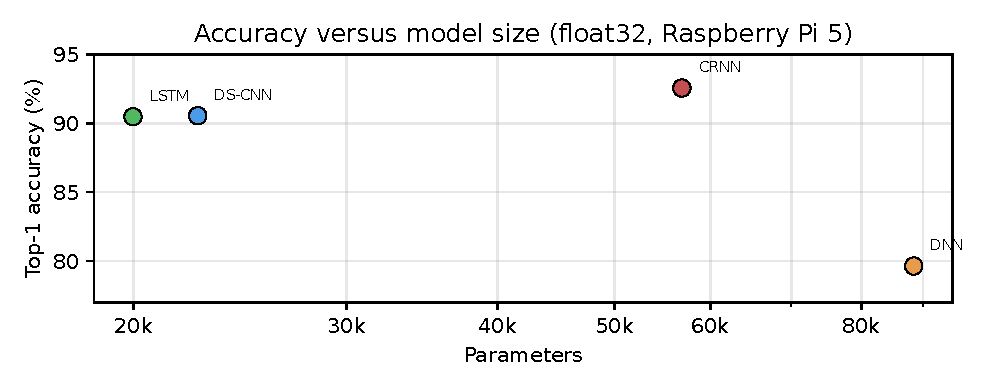
\includegraphics[width=\linewidth]{figures/acc_params.pdf}
  \end{column}

  \begin{column}{0.46\textwidth}
    \begin{block}{Architecture Selection}
      \begin{itemize}\small
        \item \textbf{CRNN (Top Accuracy)}: Highest accuracy (\textbf{92.56\%} subset, \textbf{92.08\%} full task) at 56.8k params.
        \item \textbf{LSTM (Parameter-Efficient)}: Reaches 90.48\% with only \textbf{19,980 parameters}, but higher PTQ drop.
        \item \textbf{DS-CNN (Sweet Spot)}: Optimal balance: 22.6k params, 95.49\% full task, 0.1268\,ms latency.
        \item \textbf{DNN (Baseline Anchor)}: Spends 88.4k params for lowest accuracy (72.65\% on 12-class).
      \end{itemize}
    \end{block}
  \end{column}
\end{columns}
\end{frame}

% =============================================================================
% SLIDE 10: Conclusion & Practical Guidelines
% =============================================================================
\begin{frame}{Conclusion: Practical Guidelines}
\framesubtitle{Takeaways for Edge AI Practitioners}
\begin{block}{Core Findings}
  \begin{enumerate}\small
    \item \textbf{Runtime Gap Does Not Generalize}: Defaulting to ONNX Runtime only benefits multi-threaded convolution; for dense and recurrent models, \textbf{TensorFlow Lite is 1.40--2.09$\times$ faster}.
    \item \textbf{Iso-Thread Parity Favors TFLite}: When pinned to equal thread counts ($T=1, 2, 4$), TensorFlow Lite is faster across all architectures.
    \item \textbf{Quantization Exchange Rate}: Full-int8 yields a 1.7--2.5$\times$ speedup at negligible accuracy cost, except on recurrent units (LSTM).
    \item \textbf{Race-to-Sleep Advantage}: Lower latency directly saves 35\% battery energy per inference.
  \end{enumerate}
\end{block}

\begin{alertblock}{Actionable Recommendation}
  \small \textbf{Choose your edge runtime based on architectural operator distribution, not convention.} Test both TFLite and ONNX with pinned threads before production deployment.
\end{alertblock}
\end{frame}

% =============================================================================
% SLIDE 11: Open Science & Q&A
% =============================================================================
\begin{frame}{Open Science \& Reproducibility}
\framesubtitle{ICAITech 2026 — Questions \& Comments Welcome}
\vspace{-0.2em}
\begin{center}
  {\Large\textbf{Thank You for Your Attention!}}\\[0.3ex]
  {\small\textit{Questions \& Discussion Welcome}}
\end{center}

\vspace{0.1em}
\begin{columns}[T]
  \begin{column}{0.48\textwidth}
    \begin{exampleblock}{Open Science Artifacts}
      \begin{itemize}\small
        \item \textbf{Zenodo Permanent DOI}:\\
          {\footnotesize\href{https://doi.org/10.5281/zenodo.23765521}{\texttt{10.5281/zenodo.23765521}}}
        \item \textbf{GitHub Repository}:\\
          {\footnotesize\href{https://github.com/jaweed3/kws-pi5-benchmark}{\texttt{github.com/jaweed3/kws-pi5-benchmark}}}
        \item \textbf{Open License}: GNU AGPLv3
      \end{itemize}
    \end{exampleblock}
  \end{column}

  \begin{column}{0.48\textwidth}
    \begin{block}{Contact Authors}
      \begin{itemize}\small
        \item \textbf{Fatih Jawwad Al Mumtaz}\\
          \texttt{\scriptsize fatihalmumtaz76@student.cs.unida.gontor.ac.id}
        \item \textbf{Amirul Al Aziz}\\
          \texttt{\scriptsize amirulalaziz57@student.tip.unida.gontor.ac.id}
        \item {\scriptsize Faculty of Science and Technology,\\Universitas Darussalam Gontor, Indonesia}
      \end{itemize}
    \end{block}
  \end{column}
\end{columns}
\end{frame}

\end{document}
